% adapted from https://github.com/ashishpatel26/Tools-to-Design-or-Visualize-Architecture-of-Neural-Network
\documentclass[border=15pt, multi, tikz]{standalone}
%\usepackage{blocks}
\usepackage{import}
\subimport{layers/}{init}
\usetikzlibrary{positioning}
\usetikzlibrary{3d} %for including external image 
\usetikzlibrary{decorations.pathreplacing,calligraphy}
\def\ConvColor{rgb:yellow,5;red,1.5;white,5}
\def\ConvReluColor{rgb:yellow,5;red,5;white,5}
%\def\PoolColor{rgb:red,1;black,0.3}
\def\PoolColor{rgb:green,2;black,0.3}
\def\FcColor{rgb:blue,5;red,2.5;white,5}
\def\FcReluColor{rgb:blue,5;red,5;white,4}
\def\SoftmaxColor{rgb:magenta,5;black,7}

%\tikzset{my_rectangle/.style={draw,rectangle, minimum width=2cm, minimum height=1cm}}

\begin{document}
\begin{tikzpicture}
\tikzstyle{connection}=[ultra thick,every node/.style={sloped,allow upside down},draw=\edgecolor,opacity=0.7]
%%%%%%%%%%%%%%%%%%%%%%%%%%%%%%%%%%%%%%%%%%%%%%%%%%%%%%%%%%%%%%%%%%%%%%%%%%%%%%%%%%%%%%%%
%% Draw Layer Blocks
%%%%%%%%%%%%%%%%%%%%%%%%%%%%%%%%%%%%%%%%%%%%%%%%%%%%%%%%%%%%%%%%%%%%%%%%%%%%%%%%%%%%%%%%
\node[canvas is zy plane at x=0] (testimage) at (-3.5,0,0) {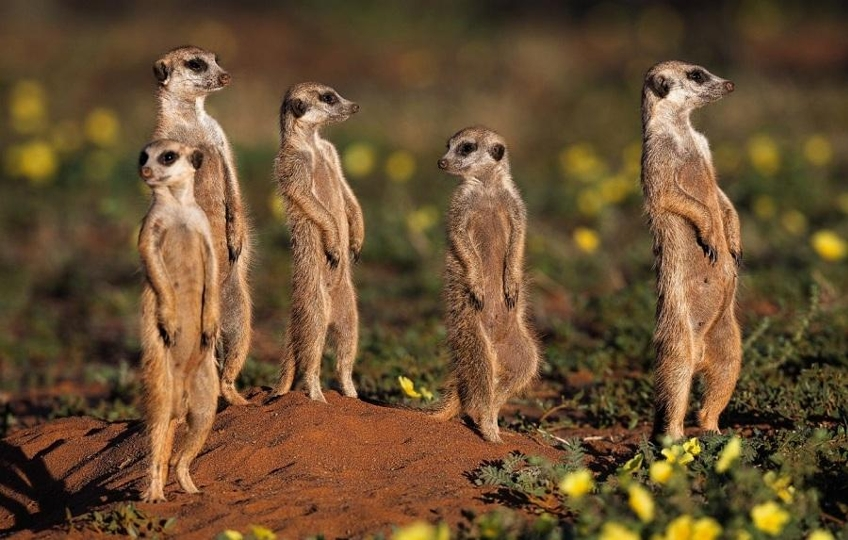
\includegraphics[width=8cm,height=8cm]{meerkatirl.jpg}};
% conv1_1,conv1_2
\pic[shift={(0,0,0)}] at (0,0,0) {RightBandedBox={name=cr1,caption=block1,%
        xlabel={{"64","64"}},ylabel=224,zlabel=224,fill=\ConvColor,bandfill=\ConvReluColor,%
        height=40,width={2,2},depth=40}};
%pool1
\pic[shift={(0,0,0)}] at (cr1-east) {Box={name=p1,%
        fill=\PoolColor,opacity=0.5,height=35,width=1,depth=35}};
%%%%%%%%%%
% conv2_1,conv2_2
\pic[shift={(2,0,0)}] at (p1-east) {RightBandedBox={name=cr2,caption=block2,%
        xlabel={{"128","128"}},zlabel=112,fill=\ConvColor,bandfill=\ConvReluColor,%
        height=35,width={3,3},depth=35}};
%pool2
\pic[shift={(0,0,0)}] at (cr2-east) {Box={name=p2,%
        fill=\PoolColor,opacity=0.5,height=30,width=1,depth=30}};
%%%%%%%%%%
% conv3_1,conv3_2
\pic[shift={(2,0,0)}] at (p2-east) {RightBandedBox={name=cr3,caption=block3,%
        xlabel={{"256","256","256"}},zlabel=56,fill=\ConvColor,bandfill=\ConvReluColor,%
        height=30,width={4,4,4},depth=30}};
    
%pool3
\pic[shift={(0,0,0)}] at (cr3-east) {Box={name=p3,%
        fill=\PoolColor,opacity=0.5,height=23,width=1,depth=23}};
%%%%%%%%%%
% split
\node[shift={(0.9,0,0)},draw,rectangle,canvas is zy plane at x=0,minimum width=12cm,minimum height=12cm,fill=blue!40!white, opacity=0.3] (sL) at (p3-east) {};

\node[shift={(-2.5,7,0)}] (spl) at (sL) {\textbf{Split at the output of block3 conv3}};
%%%%%%%%%%
% conv4_1,conv4_2,conv4_3
\pic[shift={(1.8,0,0)}] at (p3-east) {RightBandedBox={name=cr4,caption=block4,%
        xlabel={{"512","512","512"}},zlabel=28,fill=\ConvColor,bandfill=\ConvReluColor,%
        height=23,width={7,7,7},depth=23}};
%pool4
\pic[shift={(0,0,0)}] at (cr4-east) {Box={name=p4,%
        fill=\PoolColor,opacity=0.5,height=15,width=1,depth=15}};
%%%%%%%%%%
% conv5_1,conv5_2,conv5_3
\pic[shift={(1.5,0,0)}] at (p4-east) {RightBandedBox={name=cr5,caption=block5,%
        xlabel={{"512","512","512"}},zlabel=14,fill=\ConvColor,bandfill=\ConvReluColor,%
        height=15,width={7,7,7},depth=15}};
%pool5
\pic[shift={(0,0,0)}] at (cr5-east) {Box={name=p5,%
        fill=\PoolColor,opacity=0.5,height=10,width=1,depth=10}};
%%%%%%%%%%
% fc6
\pic[shift={(3,0,0)}] at (p5-east) {RightBandedBox={name=fc6,caption=fc1,%
        xlabel={{"1",""}},zlabel=4096,fill=\FcColor,bandfill=\FcReluColor,%
        height=3,width=3,depth=100}};
%%%%%%%%%%
% fc7
\pic[shift={(2,0,0)}] at (fc6-east) {RightBandedBox={name=fc7,caption=fc2,%
        xlabel={{"1","dummy"}},zlabel=4096,fill=\FcColor,bandfill=\FcReluColor,%
        height=3,width=3,depth=100}};
%%%%%%%%%%
% fc8
\pic[shift={(1.5,0,0)}] at (fc7-east) {RightBandedBox={name=fc8,caption=predictions,%
		xlabel={{"1","dummy"}},fill=\FcColor,bandfill=\FcReluColor,%
		height=3,width=3,depth=25}};

%%%%%%%%%%
% softmax
\pic[shift={(0,0,0)}] at (fc8-east) {Box={name=softmax,%
		xlabel={{"","dummy"}},zlabel=1000,opacity=0.8,fill=\SoftmaxColor,%
		height=3,width=1.5,depth=25}};

\node[shift={(3.1,0,0)}] (pred) at (softmax-east) {\textbf{``Meerkat"}};
%%%%%%%%%%%%%%%%%%%%%%%%%%%%%%%%%%%%%%%%%%%%%%%%%%%%%%%%%%%%%%%%%%%%%%%%%%%%%%%%%%%%%%%%
%% Draw Arrow Connections
%%%%%%%%%%%%%%%%%%%%%%%%%%%%%%%%%%%%%%%%%%%%%%%%%%%%%%%%%%%%%%%%%%%%%%%%%%%%%%%%%%%%%%%%
\draw [connection]  ++(-3.5,0,0)        -- node {\midarrow} (p1-west);
\draw [connection]  (p1-east)        -- node {\midarrow} (cr2-west);
\draw [connection]  (p2-east)        -- node {\midarrow} (cr3-west);
\draw [connection]  (p3-east)        -- node {\midarrow} (cr4-west);
\draw [connection]  (p4-east)        -- node {\midarrow} (cr5-west);
\draw [connection]  (p5-east)        -- node {\midarrow} (fc6-west);
\draw [connection]  (fc6-east)       -- node {\midarrow} (fc7-west);
\draw [connection]  (fc7-east)       -- node {\midarrow} (fc8-west);
\draw [connection]  (softmax-east)   -- node {\midarrow} ++(2.1,0,0);
%%%%%%%%%%%%%%%%%%%%%%%%%%%%%%%%%%%%%%%%%%%%%%%%%%%%%%%%%%%%%%%%%%%%%%%%%%%%%%%%%%%%%%%%
%% Draw Dotted Edges 
%%%%%%%%%%%%%%%%%%%%%%%%%%%%%%%%%%%%%%%%%%%%%%%%%%%%%%%%%%%%%%%%%%%%%%%%%%%%%%%%%%%%%%%%
\draw[densely dashed]
    (fc6-west)++(0, 1.5*.2, 1.5*.2) coordinate(a) -- (p5-nearnortheast)
    (fc6-west)++(0,-1.5*.2, 1.5*.2) coordinate(b) -- (p5-nearsoutheast)
    (fc6-west)++(0,-1.5*.2,-1.5*.2) coordinate(c) -- (p5-farsoutheast)
    (fc6-west)++(0, 1.5*.2,-1.5*.2) coordinate(d) -- (p5-farnortheast)
    
    (a)--(b)--(c)--(d)
    ;
    
\draw[decorate, decoration={calligraphic brace, amplitude=10pt,
	raise=5pt, mirror},line width=1pt] (-1.5, -7) -- (7.5, -7) node [midway, yshift=-1cm](edgelabel) {\textbf{Edge sub-model}};

\draw[decorate, decoration={calligraphic brace, amplitude=10pt,
	raise=5pt, mirror},line width=1pt] (8.5, -7) -- (30.5, -7) node [midway, yshift=-1cm] {\textbf{Cloud sub-model}};

\node[shift={(-7,0,0)}] (testimage) at (edgelabel) {\textbf{Test Image}};

%%%%%%%%%%%%%%%%%%%%%%%%%%%%%%%%%%%%%%%%%%%%%%%%%%%%%%%%%%%%%%%%%%%%%%%%%%%%%%%%%%%%%%%%
\end{tikzpicture}
\end{document}
